\section{System model}
Cost, availability and on-demand scaling have accelerated customer adoption of different application deployment models - On-Premise cloud, Private cloud, Public cloud or hybrid clouds. Depending on the services that an application depends on, the choice of platform varies. A single application could potentially be reliant on multiple clouds for the set of services it consumes. From a customer/tenant perspective, monitoring service levels that their workloads are getting often becomes a complex task of aggregating information across multiple cloud providers, each using different proprietary monitoring and management stacks. Further aggravating the problem is the devops transition. Applications and consequently their bindings to services are seeing an increased rate of change. 
\begin{figure}[H]
\centering
 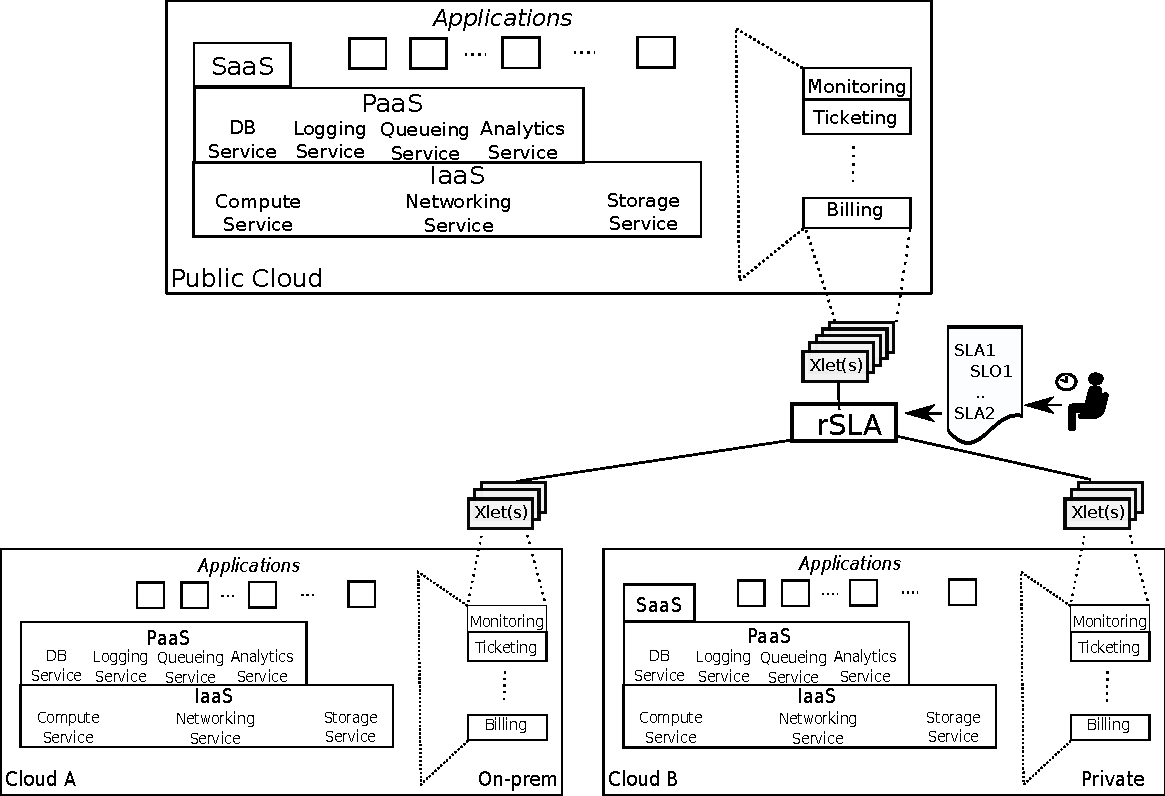
\includegraphics[width=8cm,height=8cm]{pics/systemModel.pdf} 
 \caption{rSLA System Overview}
 \label{fig:systemModel}
\end{figure}
%\todopramod{Examples for Iaas,Paas,Monitoring,Ticketing systems - variety}
Figure \ref{fig:systemModel} shows an overview of the proposed rSLA system model. rSLA is made up three main components - a language for administrators or service providers to express service level agreements, a modular SLA evaluation framework, and a set of Xlets - light weight dynamically bound adapters. The rSLA framework itself can be deployed in any of the cloud deployment models - On-Premise cloud, Private cloud, Public cloud or hybrid clouds. Section \ref{} provides a high-level overview of the rSLA language. Section \ref{} provides an overview of rSLA evaluation framework and the XLet framework. Section \ref{} discusses a case studies of rSLA deployment.

